\documentclass[tikz]{standalone}
\begin{document}
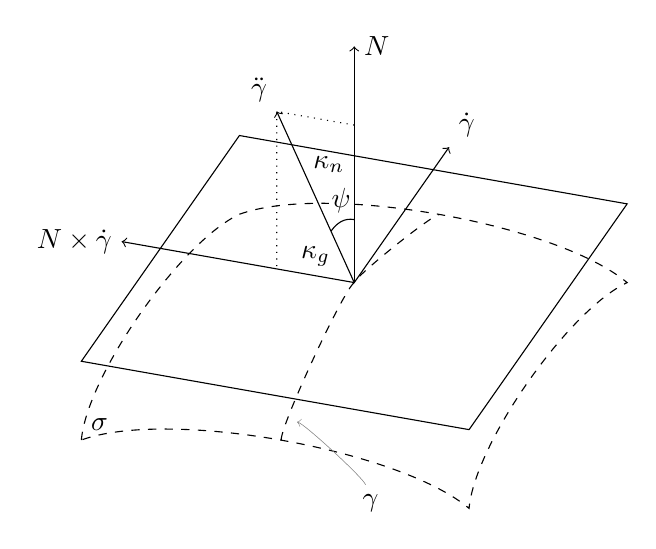
\begin{tikzpicture}[x={(170:1cm)},y={(55:.7cm)},z={(90:1cm)}]
  \draw (2.5,-2.5,0) -- (2.5,2.5,0) -- (-2.5,2.5,0) -- (-2.5,-2.5,0) -- cycle;
  \draw[dashed,looseness=.6] (2.5,-2.5,-1) node[above right] {$\sigma$}
  to[bend left] (2.5,2.5,-1)
  to[bend left] coordinate (mp) (-2.5,2.5,-1)
  to[bend right] (-2.5,-2.5,-1)
  to[bend right] coordinate (mm) (2.5,-2.5,-1)
  -- cycle;
  \draw[dashed,looseness=.2] (mm) to[bend left] (0,0,0) to[bend left] (mp);
  \path[looseness=.2] (mm) to[bend left]
  node[pos=.2,pin={[pin distance=1cm,pin edge={solid,<-}]below right:$\gamma$}] {} (0,0,0);

  \draw[->] (0,0,0) -- (3,0,0) node[left] {$N\times\dot{\gamma}$};
  \draw[->] (0,0,0) -- (0,3,0) node[above right] {$\dot{\gamma}$};
  \draw[->] (0,0,0) -- (0,0,3) node[right] {$N$};
  \draw[dotted] (0,0,2) -- (1,0,2) -- (1,0,0);
  \draw[->] (0,0,0) -- coordinate[pos=.3] (psi) (1,0,2) node[above left] {$\ddot{\gamma}$};
  \node[left] at (0,0,1.5) {$\kappa_n$};
  \node[above] at (.5,0,0) {$\kappa_g$};
  \draw (0,0,.8) to[out=170,in=55] node[above,fill=white,inner sep=1pt,outer sep=2pt] {$\psi$} (psi);
\end{tikzpicture}
\end{document}